%Fall 2014 -- Tree walker paper
\documentclass[times]{speauth}
\bibliographystyle{wileyj}
\usepackage{listings}
\lstset{basicstyle=\tiny\ttfamily,columns=fullflexible,keepspaces=true}
\usepackage[colorlinks,bookmarksopen,bookmarksnumbered,citecolor=red,urlcolor=red]{hyperref}

\newcommand\BibTeX{{\rmfamily B\kern-.05em \textsc{i\kern-.025em b}\kern-.08em
T\kern-.1667em\lower.7ex\hbox{E}\kern-.125emX}}

\def\volumeyear{2014}

\begin{document}
\runningheads{B. Durkee, D. T. Welch, and M. Sitaraman}{Software Evolution and the Visitor Pattern: Motivation}
\title{Software Evolution and the Visitor Pattern: Motivation for a Dynamic Tree Walker}

\author{Blair Durkee\corrauth, Daniel T. Welch, Murali Sitaraman}
\address{School of Computing, Clemson University, South Carolina, SC, 
 29634, USA}

\corraddr{Blair Durkee, School of Computing, Clemson University, Clemson SC, 29631, USA.}

% -----------------------------------------------------------------------------------------------
%	Abstract
% -----------------------------------------------------------------------------------------------

\begin{abstract}
This paper describes our experiences re-engineering legacy software leading up to, and resulting in the creation of a reusable, reflection-based (dynamic) tree traversal mechanism. The mechanism we describe has come to play a central role in an ongoing software engineering project that that has slowly evolved from a relatively simple language translator, to a sophisticated verifying compiler over a period of nearly fifteen years. The source language we discuss is RESOLVE (Reusable Software Language with Verification): A `research language' designed for formal specification and verification of object-oriented programs. Being at its core a research language,  frequent and continual language-level evolution posed major maintainability challenges to the compiler. Everything from major to minor syntax changes (or additions) would often necessitate compiler wide refactors, spanning the abstract syntax representation, to the logic dictating abstract syntax traversal and all associated subcomponents. Given the development bottleneck posed by this propagation, we decided to build a novel, reflection based, generic walker that utilizes a relatively common pre-post variation of the visitor pattern. We describe this walker, some improvements to its initial design, and conclude with an application, illustrating its important role in code generation for RESOLVE's multiple target languages (C and Java). 

\end{abstract}
\keywords{visitor; design pattern; compiler; language translation}

\maketitle
\vspace{-6pt}

% -----------------------------------------------------------------------------------------------
%	Introduction
% -----------------------------------------------------------------------------------------------

\section{Introduction}
\vspace{-2pt}
Reusability and maintainability are key nonfunctional characteristics of well-engineered software. As far as long-running academia based research software projects are concerned, these qualities become especially important, but unfortunately, are too often overlooked in favor of rapid fire development -- usually culminating with that long sought-after paper or dissertation. Here we describe our solution to overcoming our system's (the RESOLVE compiler's) highly entrenched, non-reusable, and overall difficult-to-maintain preexisting tree walking strategy -- a solution which does not compromise rate of development. To understand the context in which this component was designed, and the full implications of its usage, we start with a brief overview of the compiler and its source language.

RESOLVE is an integrated programming and specification language that seeks to realize the grand challenge of software verification. By writing reusable components that are formally specified, the compiler uses these specifications to produce a number of verification conditions (VCs) for any code programmers might write. These VCs are then sent off to an integrated prover which then attempts to automatically establish each VC generated -- thus proving the program correct\footnote{\textit{All} VCs must be established to ensure program correctness.}. While this process cannot guarantee software that is specified correctly, it rules out implementation errors by proving programs correct with respect to a given specification.

The compiler, verification, and proof tools have been researched and developed over the course of many years, and successive generations of students. These tools have evolved and changed significantly, though many early design decisions still persist. One example is the mechanism used to traverse the abstract syntax tree (AST) that represents parsed RESOLVE code. As with any compiler, this logic is a key component used in multiple stages of compilation such as pre-processing, population, analyzing, semantic checking, translation, etc. The initial implementation of AST traversal worked sufficiently well, but turned out to be an impediment to the continued evolution of the compiler -- serving as motivation for the development of a dynamic tree walker to replace this older mechanism.

\vspace{-6pt}

% -----------------------------------------------------------------------------------------------
%	Related Work
% -----------------------------------------------------------------------------------------------

\section{Related Work}
\vspace{-2pt}

Since the emergence of the first compiled, high level languages, ASTs and tree traversal patterns have garnered both an extensive amount of study, and a large (still growing) body of literature. While the concept of ASTs and their usage is well established, AST construction, reusability, and long term maintenance remain relevant topics in the software engineering community [cite?]. In this section, we consider several existing parsing tools capable of generating ASTs emphasizing the maintainability cost of using such tools, and any potential mechanisms they might provide for AST traversal.

The first tool we consider is the popular GNU ``compiler compiler," Bison\footnote{Bison serves as the modern successor to the original tool that originated in the early 1970s, YACC (Yet Another Compiler Compiler)} \cite{levine:1992}. Provided with a formal grammar, this tool -- commonly referred to as a ``parser generator" -- produces a state machine capable of recognizing sentences in a given language. By annotating grammar rules with semantic actions, users are able to construct their own AST representations from the underlying concrete syntax tree implicitly shaped by the grammar rules. There are several disadvantages to Bison's approach. The first is that Bison does not provide any built in support for tree traversal: Once the AST is built, users must traverse the tree either via their own visitor, or small recursive `evaluate' methods. The second disadvantage is that developers must learn a specific, specialized Bison syntax (separate from its BNF style grammar syntax) to specify semantic actions. A third disadvantage concerns modularity: The need to annotate grammar rules with specific semantic actions inherently couples a grammar more closely to a given application. This coupling not only decreases the reusability of a grammar, but also makes it harder to maintain over time since every iteration to the rules of the grammar requires changes to the actions as well.

%Another tool building on the work of YACC/Bison is demonstrated by SableCC [2]. SableCC provides the tools necessary to convert a BNF grammar into Java packages for lexing, parsing, and tree analysis. In addition, it creates a Java class for each node in the AST. The analysis package defines an abstract class which allows for efficient and foolproof implementation of tree traversal logic. The process of parsing the code and walking the tree is all done by generated code, and the developer needs only to implement specific visitor methods to create the analysis and code generation portions of the compiler.

Another representative tool we consider is ANTLR (Another Tool for Language Recognition). Until recently, ANTLR, similar to Bison, relied upon 

is yet relied upon grammar actions and rewrite rules. with operators (distinct from actions) that  with ANTLR v4, grammars were able to be annotated with syntax controlling the s

Actively maintained by 

While the  The compiler discussed in this paper is based on ANTLR v3, upgraded from previous versions. While ANTLR v4 offers a new approach incorporating sax-dom event style parse tree listeners, we needed a quicker turnaround time than re-writing the grammar and significant portions of the compiler would allow. While there have been many innovations int he field of compiler tree walking, this paper is more specifically about the use of Java reflection to quickly allow more flexibility in accessing an existing tree structure.

% -----------------------------------------------------------------------------------------------
%	Motivation
% -----------------------------------------------------------------------------------------------

\section{Initial Implementation and Motivation}
The pipeline for compiling high-level code begins with lexing, parsing, and building an AST. This data structure is a logical representation of the source code, and it will be used in nearly every subsequent stage of the compilation pipeline. The need to traverse the tree in each stage presents a potential problem of code duplication. the traversal method will not change, but separating it from the logic of the populator, analyzer, and other components is a non-trivial task. This task, however, was simplified by a widely accepted design pattern from the gang of four \cite{gamma:1995}. This ``visitor" pattern was used, albeit imperfectly, in the initial development of the RESOLVE compiler.

The design of the tree traversal component's first iteration bears close resemblance to the visitor pattern: Each class representing a type of node in the syntax tree contains a \texttt{accept} method which can dispatch the appropriate logic through polymorphism. However, the algorithm for traversal was not properly separated from the data structure as the visitor pattern requires.

The purpose of the visitor pattern is to decouple a data structure from the logic operating on it. While manifestations of this pattern may vary, they must necessarily adhere to that specific design principle of separation. During the initial development of the RESOLVE compiler, a few shortcuts were made to solve surface issues with the visitor implementation. \ref{fig:flawedvisitorexample} illustrates a snipped of the resulting code.

\begin{figure}
\centering
\begin{minipage}{.45\textwidth}
\begin{lstlisting}[language=java]
public abstract
	class ResolveConceptualVisitor {
    visitProcedureDecl(
    		ProcedureDecl e) {}
}

public abstract 
	class ResolveConceptualElement {
    abstract void accept(
        ResolveConceptualVisitor e);
}

public class ProcedureDecl
	extends ResolveConceptualElement {	
    List<Stmt> myStatements;
    
    public void accept(
    		ResolveConceptualVisitor e) {
        v.visitProcedureDecl(this);
    }
}
\end{lstlisting}
\end{minipage}\quad
\begin{minipage}{.45\textwidth}
\begin{lstlisting}[language=java]
public class Analyzer
	extends ResolveConceptualVisitor {
	
    public void visitProcedureDecl(
  			ProcedureDecl e) {
        table.beginProcedureScope();
        visitStmtList(e.getStatements();
	table.endProcedureScope();
    }
    
    private void visitStmtList(
    		List<Stmt> e) {
        for (Stmt s : e.getStatements()) {
            visitStmt(s);
        }
    }
    
    public void visitStmt(Stmt e) {
        e.accept(this);
    }
}
\end{lstlisting}
\end{minipage}
\caption{A flawed implementation of the visitor pattern.}
\label{fig:flawedvisitorexample}
\end{figure}

The traversal logic, according to visitor pattern, should be contained within the \texttt{accept} visitor method. In this initial implementation, it has been moved to the visit method contained in the \texttt{ResolveConceptualVisitor} component. Consequently, every \texttt{ResolveConceptualVisitor} will bear the responsibility of traversing the syntax tree. Thus, most changes in the trees structure, no matter how minor, necessitates large, cross component refactors.

\begin{figure}[!htb]
\centering
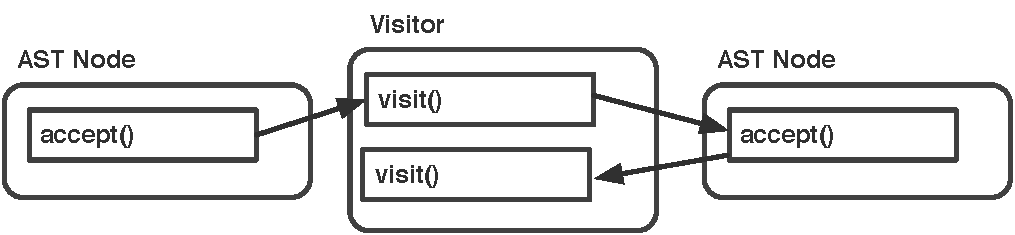
\includegraphics[scale=.60]{figures/flawed_visitor_organization.pdf}
\caption{A high level look at the organization of the flawed visitor.}
\label{fig:flawedvisitororganization}
\end{figure}

The reason for the appearance of this critical flaw is unknown, but it seems likely to be related to the singular visit method rather than pre-post traversal visits. Consider the same code with that minor change, shown in \ref{fig:fixedvisitorexample}

\begin{figure}[!htb]
\centering
\begin{minipage}{.45\textwidth}
\begin{lstlisting}[language=java]
public abstract
	class ResolveConceptualVisitor {
    preProcedureDecl(ProcedureDecl e) {}
    postProcedureDecl(ProcedureDecl e) {}
}

public abstract 
	class ResolveConceptualElement {
    abstract void accept(
        ResolveConceptualVisitor e);
}

public class ProcedureDecl
	extends ResolveConceptualElement {	
    List<Stmt> myStatements;
    
    public void accept(
    	  ResolveConceptualVisitor e) {
        v.preProcedureDecl(this);
        for (Stmt s : e.getStatements()) {
            s.accept();
        }
        v.postProcedureDecl(this);
    }
}
\end{lstlisting}
\end{minipage}\quad
\begin{minipage}{.45\textwidth}
\begin{lstlisting}[language=java]
public abstract class Stmt
	extends ResolveConceptualVisitor {
    abstract void accept(
    	ResolveConceptualVisitor e) {}
}

public class Analyzer
	extends ResolveConceptualElement {
	
    public void preProcedureDecl(
  			ProcedureDecl e) {
        table.beginProcedureScope();
    }
    
    public void postProcedureDecl(
    			ProcedureDecl e) {
        table.endProcedureScope();
    }        
}
\end{lstlisting}
\end{minipage}
\caption{A flawed implementation of the visitor pattern.}
\label{fig:fixedvisitorexample}
\end{figure}

\begin{figure}[!htb]
\centering
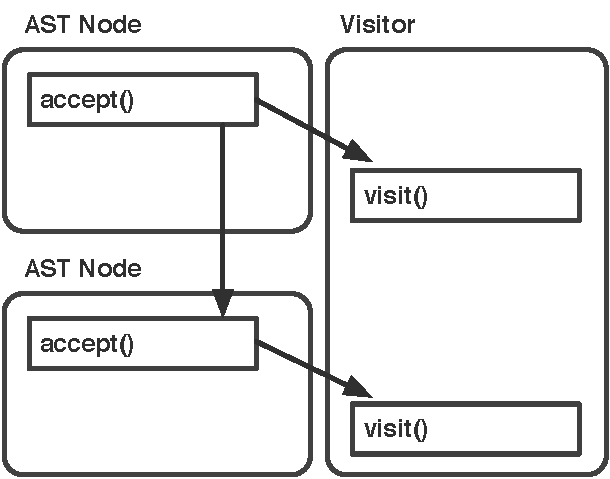
\includegraphics[scale=.60]{figures/fixed_visitor_organization.pdf}
\caption{A high level look at the organization of the fixed visitor.}
\label{fig:fixedvisitororganization}
\end{figure}

The \texttt{ResolveConceptualVisitor} now has fewer methods and the traversal logic is properly decoupled from the visitor logic.

% -----------------------------------------------------------------------------------------------
%	Contribution
% -----------------------------------------------------------------------------------------------

\section{A Dynamic Tree Walker}
While the corrections demonstrated in \ref{fig:fixedvisitororganization} could be made, we decided to pursue a third, even more robust implementation that would exist independently of--and work simultaneously with--existing code. We created an entirely new class simply named TreeWalker. This new traversal component is completely decoupled from the data structure and dynamically analyzes the structure at runtime using Java reflection.

Instead of reusing the existing ResolveConceptualVisitor class, we created a new abstract visitor class for the dynamic tree walker--TreeWalkerVisitor. This decision allows the legacy code to continue to work alongside the new dynamic traversal component. One tradeoff is that future visitors have to be entirely rewritten (or at least heavily refactored), but the concern is mitigated, as old components can continue to work until the new components are ready to be dropped in place.

With two new components in place, the Tree Walker can then call the visitor methods as it traverses the tree. \ref{fig:newvisit} is a simplified version of the traversal algorithm.

\begin{figure}[!htb]
\centering
\begin{minipage}{.80\textwidth}
\begin{lstlisting}[language=java]
public void visit(ResolveConceptualElement e) {
    invokeVisitorMethods("pre", e);
    
    for (ResolveConceptualElement node : e.getChildren()) {
        visit(node);
    }
    invokeVisitorMethods("post", e);
}
\end{lstlisting}
\end{minipage}
\caption{A revised \texttt{visit} method.}
\label{fig:newvisit}
\end{figure}

The \texttt{visit} method is a simple recursive, depth-first traversal of the AST. At each level, the procedure will make ``pre" call before visiting children, and a ``post" call after. These calls are made via \texttt{invokeVisitorMethods} -- a local method used to construct the appropriate visitor name and dispatch the correct call using reflection techniques.

\begin{figure}[!htb]
\centering
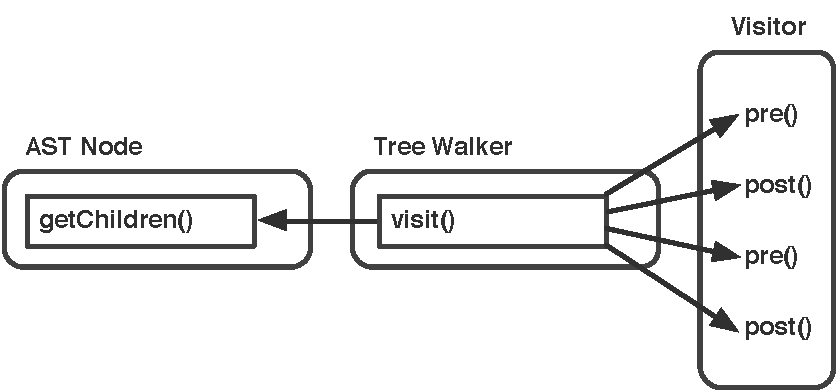
\includegraphics[scale=.60]{figures/prepostprepost.pdf}
\caption{A revised \texttt{visit} method.}
\end{figure}

The logic for retrieving a node's children is contained in the \texttt{getChildren} defined in the root RESOLVEs AST hierarchy, the \texttt{ResolveConceptualElement} class. This design choice allows for more control over the method of traversal. The default method uses Java reflection to obtain a list of the children for a given node, and the children are returned in a list of unspecified order. If the order is important (or needs to be different from the default), then inheriting classes can override the method with hard-coded logic for returning the children. Figure 4 shows a simplified version of this method.

\begin{figure}[!htb]
\centering
\begin{minipage}{.80\textwidth}
\begin{lstlisting}[language=java]
public List<ResolveConceptualElement getChildren() {
    List<ResolveConceptualElement> children = new LinkedList<>();
    ArrayList<Field> fields = new ArrayList<>();
    
    //Populate "fields" with the declared fields of the object's defining class
    
    Iterator<Field> iterFields = fields.iterator();
    while(iterFields.hasNext()) {
        Field curField = iterFields.next();
        
        Class<?> fieldType = curField.getType();
        if (ResolveConceptualElement.class
                  .isAssignableFrom(fieldType)) {
            children.add(ResolveConceptualElement
                .class.cast(curField.get(this)));
        }
    }
}
\end{lstlisting}
\end{minipage}
\caption{An implementation of \texttt{getChildren}.}
\label{fig:getchildren}
\end{figure}


The visitors we use include a number of typical compiler components and are indicated in \ref{fig:getchildren}. Each visitor can override as many or as few visit methods as needed, making the creation of a new visitor quite simple. this has many advantages for maintainability as well. Unlike the original implementation of the visitor pattern, the tree walker allows new methods to be added to a visitor without the need to consider existing code. All the traversal logic is contained within the tree walker class. 

% -----------------------------------------------------------------------------------------------
%	Application
% -----------------------------------------------------------------------------------------------

\section{Application: Code Generation}
\vspace{-2pt}

One application of the walking mechanism that has been described at length in this paper is its key role in RESOLVE's code generation phase. Since development began on the compiler, code generation -- like the many other phases of compilation -- was hindered not only by initial design of the AST visitor, but also by the (unusually) steep set of constraints RESOLVE code generation is subject to, including the following.

\begin{enumerate}
\item \textit{Correct by construction}: Provided with successfully verified RESOLVE source-code, it falls upon the translator to model, as faithfully as possible, each construct of the source language \textit{within} the target language. This modeling process -- which strives to maintain the established correctness of the original source -- typically precludes the possibility of any sort of syntax-directed translation -- as any code generated fitting such a model inevitably ends up looking wildly different from the original source.
\item \textit{Extensibility}: The design of the translator must allow users to relatively easily tweak the output of a given construct, add support for altogether new constructs (accounting for the rapidly developing nature of the source language), and not preclude the addition of any future target languages. This is ultimately one of the reasons we choose to perform source-to-source translation, as opposed generating byte code such as JVM or LLVM single static assignment form directly: It allows a certain level of flexibility -- leaving us free to temporarily sidestep the non-trivial problem of developing (and maintaing) a fully blown byte level interpretation of every RESOLVE construct, in favor of more fruitful, verification related avenues of research.
\item \textit{Reusability}: If two or more supported target languages share similar constructs, the (separate) modules responsible for generating code for each should not duplicate code. Rather, they would ideally be designed to share as much common translation logic as possible, typically via an abstract class or some other means. However, if this is to occur, the translator in question must be designed in such a way that it enforces a strict separation between the logic governing the collection of translation related information, and the actual formatted output of this information.
\end{enumerate}

With these requirements in place, development of a RESOLVE translator hinges on two key pieces: A mechanism for traversing RESOLVE's AST efficiently and automatically (detailed in this paper), and the ability to efficiently separate translation \textit{information collection logic} from translation \textit{output logic}. In this section, we detail -- by way of a small example -- our approach which utilizes the pre-post methods of the tree walker and the ANTLR tool \textit{StringTemplate} to help us maintain the necessary separation between the model of our translation and view responsible for output.

To illustrate the general process of producing runnable C from RESOLVE, consider the following simple operation:

\begin{verbatim}
Operation Int_Do_Nothing(); 
Procedure
        Var X : Integer;
        X := 3;
end Nothing;
\end{verbatim}

Shown in \ref{fig:translationflow} is a high level depiction of the steps taken in translating this operation to C. The first box depicts the AST of operation \texttt{Int\_Do\_Nothing}, where nodes are represented as boxes labeled by the constructs they contain. Throughout the walk of the tree, useful information such as the operation's name ``Int\_Do\_Nothing" are extracted from the nodes, and added as parameters to user defined templates\footnote{A template can simply be thought of as a ``document with holes" which the user choses when and how to fill.}, in this case: \texttt{c\_function\_def}.

\begin{figure}
\centering
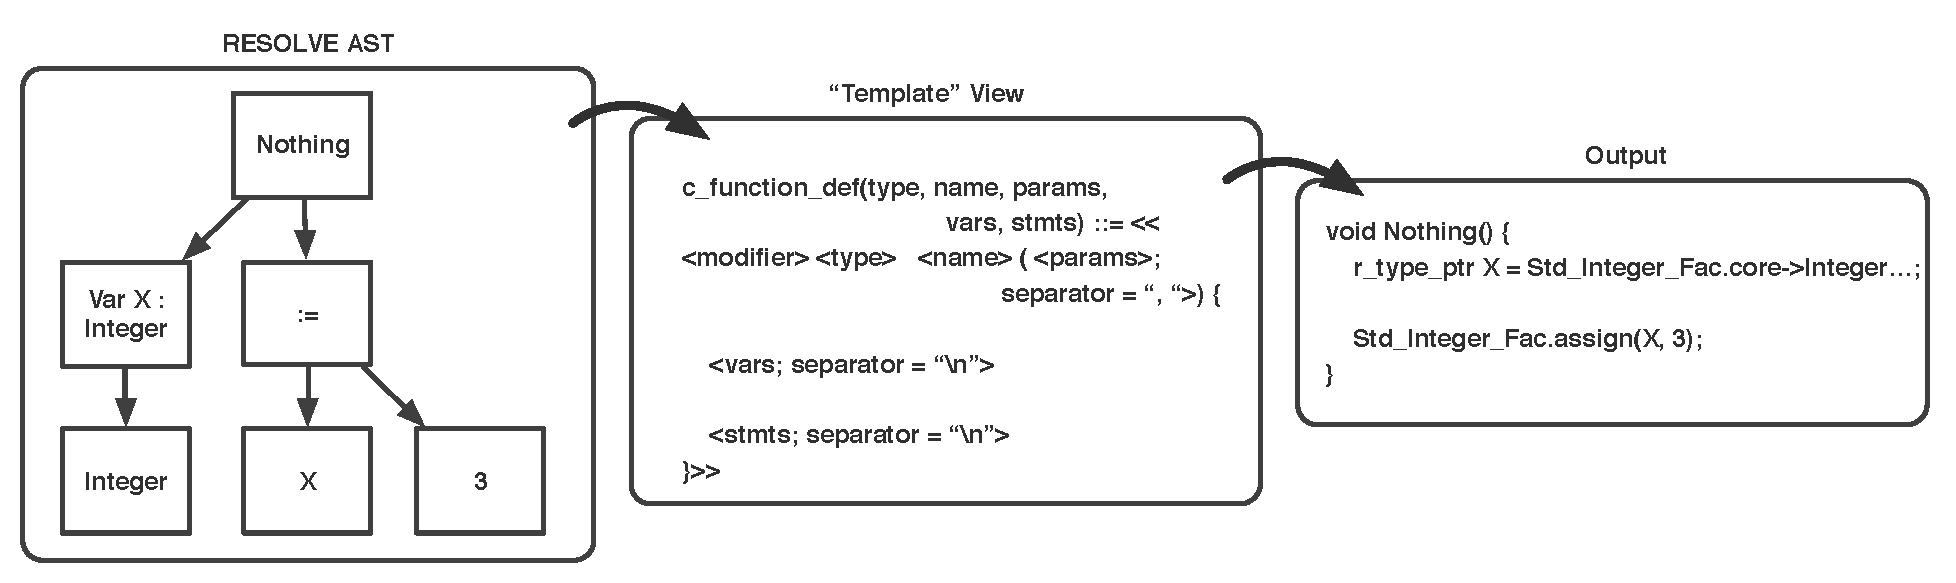
\includegraphics[scale=.40]{figures/ast_traversal2.pdf}
\caption{The general flow of information from the AST (first), to user defined templates (middle), ending with formed output (last).}
\label{fig:translationflow}
\end{figure}

In the context of RESOLVE to C translation, these templates, when filled during the aforementioned pre-post visitor traversal of RESOLVE's AST, help simplify the task of producing arbitrarily complicated, nested blocks of structured C output by keeping translation logic strictly with the C translator, and output logic strictly within the templates.

That is, the only actual work being performed within the C translator is forwarding information collected from individual \texttt{ResolveConceptualElement}s, to a series of externally defined templates. This allows us to exploit (in design pattern parlance) a strict model view controller (MVC) separation in the translator's codebase between the mechanism that does the AST visiting (controller), the individual \texttt{ResolveConceptualElement}s from which we're adding information to templates (model), and the external file containing all available C language templates which shape our output (view) \cite{krasner:1988}.

We feel the approach to tree walking in the paper lends itself well to this strategy of translation, as this separation allows us to easily iterate changes to our generated C (or Java!) code without needing to concern ourselves with the compiler or translator itself.

% -----------------------------------------------------------------------------------------------
%	Conclusion
% -----------------------------------------------------------------------------------------------

\section{Conclusion}

% -----------------------------------------------------------------------------------------------
%	Acknowledgments
% -----------------------------------------------------------------------------------------------

\section{Acknowledgements}

\bibliography{treewalkreferences}

\end{document}
